\chapter{Data Acquisition}
To record audio, one might need to use a microphone. A microphone generates an analog electric signal, but to analyse this electric signal it needs to be digitised. In this chapter it is described how to digitise an audio signal.\\
In \autoref{fig:mic_AD_MCU_PC} a generalised view of the setup, used in this project, is illustrated.

\begin{figure} [H]
    \centering
 \newcommand{\microphone}{%
    \tikz{
        \begin{scope}
            \clip (-.3em,-.4ex) rectangle (1.3em,1.5ex);
            \fill[black, rounded corners=1.5ex] (-.3em,-.4ex) rectangle (1.3em,5.5ex);
        \end{scope}
        \fill[white, rounded corners=1.3ex] (-.1em,0) rectangle (1.1em,5.1ex);
        \fill[black, rounded corners=1.1ex] (0,.2ex) rectangle (1em,5ex);
        \foreach \pos in {2.5ex, 2.9ex, 3.3ex, 3.7ex}
            \fill[white, rounded corners=.1ex] (.35em,\pos) rectangle +(.8em,.25ex);
        \fill[black] (.4em,-.4ex) rectangle (.6em,-1.5ex);
        \fill[black] (0,-1.5ex) rectangle (1em,-2ex);
    }%
}
    \tikzstyle{frame} = [
        rectangle, draw, 
        text width=5em, text centered,
        minimum height=4em
    ]
    \tikzstyle{line} = [draw, -latex']
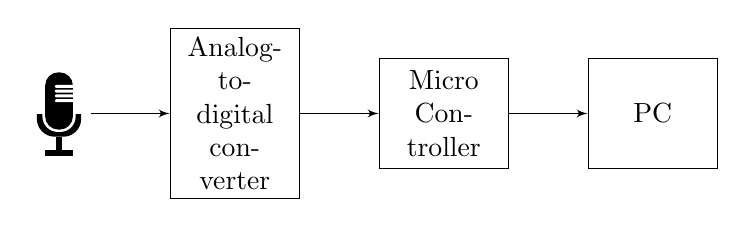
\begin{tikzpicture}[node distance = 4cm]
    \node [frame] (A/D) {Analog-to-digital converter};
    \node [left=1cm of A/D] (mic) {\microphone};
    \node [frame, right=1cm of A/D] (mcu)  {Micro Controller};
    \node [frame, right=1cm of mcu] (pc)  {PC};


    \path [line] (mic) -- (A/D);
    \path [line] (A/D) -- (mcu);
    \path [line] (mcu) -- (pc);
  
\end{tikzpicture}
    \caption{Flowchart...} 
    \label{fig:mic_AD_MCU_PC}
\end{figure}


\section{Microphone}
Microphones are used to convert sound into an electric signal. This is done by converting oscillations in the air into an oscillating electric signal. 

\begin{figure}[H]
    \centering
    \includegraphics[scale=0.65]{figures/Microphone_figure.png}
    \caption{A figure of a simplified electret microphone \cite[p. 160]{LectureNotes}.}
    \label{fig:mic_figure}
\end{figure}

\autoref{fig:mic_figure} shows a simplified version of an electret microphone. The electret microphone works as follows: When a sound wave is going through the dust cover the electret diaphragm will begin to oscillate. When this happens there will be a change in the distance between the backplate and the diaphragm. When the distance changes between the diaphragm and the backplate, the capacitance changes, thus will the charge on the backplate. This causes a change in voltage between the diaphragm and the backplate and is detected by the field effect transistor, which then amplifies the signal.

\noindent The diaphragm and the backplate acts as a capacitor and can be described as
\begin{align}
    C = \dfrac{\varepsilon A}{d}, \label{eq:capacitance}
\end{align}
where $\varepsilon$ is the permittivity (a measure of the electric polarisation of the electrical insulator), $A$ is the area of the plates and $d$ is the distance between the diaphragm and the backplate. $A$ and $\varepsilon$ are considered constants. $d$ can be described as the distance between the diaphragm and the backplate at time $t$, hence $C$ becomes a function of $d(t)$. The voltage between the plates and their charge has the relation:
\begin{align}
q(t)=C v_C(t).
\label{eq:ChargeAtTime}
\end{align}
Using \eqref{eq:capacitance} and \eqref{eq:ChargeAtTime} it yields:
\begin{align*}
    v_C(t)=v_C(d(t))= \dfrac{q(t)}{C(d(t))} = \dfrac{q(t)d(t)}{\varepsilon A},
\end{align*}
where $v_C$ is the voltage between the plates. This means that when $d$ decreases, the charge on the diaphragm induces an increased charge on the backplate. 
\cite[p. 160-161]{LectureNotes}

\section{Signals}
A purpose for signals is to carry information about physical phenomenons. Signals can be represented mathematically as a function with one or more independent variables. The information described by the signal could be how specific systems act. An examples of a signal could be a speech signal, which is acoustic pressure as a function of time. Signals are represented in two ways, continuous- and discrete signals. Continuous signals are defined by continuance of values of the independent variable, whereas discrete signals are defined at discrete times, where the independent variables are discrete set of values. \cite[p. 1-4]{signalSystems} 


\section{Discrete Signals} \label{sec:discrete_signal}
\begin{figure} [H]
    \centering
    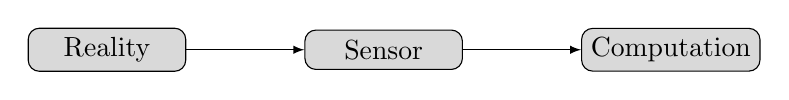
\begin{tikzpicture}[
    node distance = 15mm,
every node/.style = {draw=black, rounded corners, fill=gray!30, 
                     minimum width=2cm, minimum height=0.5cm,
                     align=center},
every path/.style = {draw, -latex}
                        ]
\node (Sensor) {Sensor};
\node (Reality) [left=of Sensor]       {Reality}; 
\node (Computation) [right=of Sensor]     {Computation};

\draw   (Reality) -- (Sensor);
\draw   (Sensor) -- (Computation);
    \end{tikzpicture}
    \caption{A figure showing the interactions between the physical reality and computing} %better caption
    \label{fig:reality_computing}
\end{figure}
When working with discrete signals, an essential thing is to look at sampling. By sampling a signal it can then be stored and analysed in a digital computer. From  \autoref{fig:reality_computing}, sampling is necessary to come from the sensor part to the computing part.

\subsection*{Discrete-time Signals} 
Working with recorded audio, which is a continuous-time signal, it can be beneficial to consider it in discrete time instead.
Going from a continuous-time signal, $x_c(t)$, to a discrete-time signal, $x[n]$, the discrete-time signal can be manipulated by a computer. A discrete-time signal is essentially a sampled continuous-time signal.

A typical way to obtain a discrete-time signal from a continuous-time signal is by using periodic sampling. A periodic sampling is a sequence of samples, $x[n]$, also referred to as the n'th sample, obtained from the continuous-time signal, $x_c(t)$, by using the following relation:
\begin{align*}
x[n]=x_c (nT), \quad   n \in \mathbb{Z},
\end{align*}
where $T$ is the sampling period and it is from the relation $f=\dfrac{1}{T}$, where $f$ is the sampling frequency, in samples per second. This can also be called a C/D converter, ideal continuous to discrete converter. 
By using a A/D converter, analog to digital converter, an approximation of the C/D conversion is achieved. \cite[p. 140-142]{DiscreteTimeSignal}\\

\section{Sampling}

\usetikzlibrary{shapes,arrows}
    \usetikzlibrary{positioning}
    
\begin{figure} [H]
    \centering
    \tikzstyle{frame} = [
        rectangle, draw, 
        text width=4em, text centered,
        minimum height=4em
    ]
    \tikzstyle{line} = [draw, -latex']
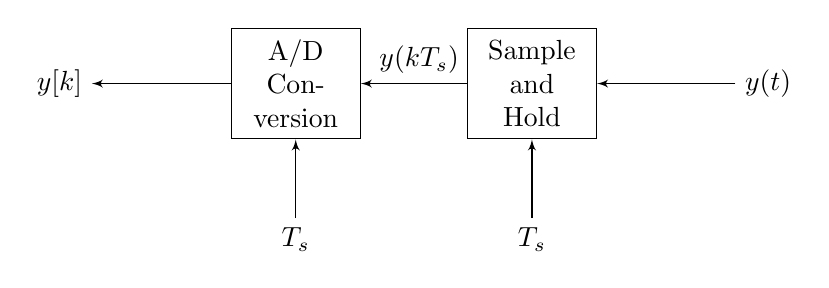
\begin{tikzpicture}[node distance = 3cm]
    \node [frame] (A/D) {A/D Conversion};
    \node [left of=A/D] (yk) {$y[k]$};
    \node [frame, right of=A/D] (SH)  {Sample and Hold};
    \node [right of=SH] (yt)  {$y(t)$};
    \node [below=1cm of SH] (ts)  {$T_s$};
    \node [below=1cm of A/D] (TS)  {$T_s$};

    \path [line] (A/D) -- (yk);
    \path [line] (SH) -- node[above,pos=.45] {$y(kT_s)$} (A/D);
    \path [line] (yt) -- (SH);
    \path [line] (ts) -- (SH);
    \path [line] (TS) -- (A/D);
\end{tikzpicture}
    \caption{A figure of the analog to digital converter....} 
    \label{fig:reality_computing}
\end{figure}

In \autoref{sec:discrete_signal} it was established that a continues signal $y(t)$ can be represented as a discrete sequence $y[t]$ of samples with a sample period $T$.\\
It is often desirable to reconstruct a signal from the discrete sequence. To do so the sequence must be uniquely determined. Whether or not a discrete sequence is uniquely determined depends on two parameters, the sample period and the bandwidth of the original signal. The bandwidth is the maximum frequency of a signal. This is possible to determine since the frequency is often bounded in practice.   

\begin{theorem}{Nyquist-Shannon Theorem}
    \label{the:Nyquist-Shannon}
    Let $f_N$ denote the bandwidth of a signal $y(t)$ then in order for the samples $y[k]$ to be uniquely determined, the sample frequency $f_s$ must satisfy:
    \begin{align*}
        f_s \geq 2f_N.
    \end{align*}
    \cite[397]{mandal2007continuous}
\end{theorem}

\noindent An example of when a series of samples are not determined, is show on \autoref{fig:aliasing}. 

\begin{figure}[H]
    \centering
    \includegraphics[width=0.9\textwidth]{figures/aliasingFig.pdf}
    \caption{The top plot is a $0.9\si{Hz}$ sine wave (in blue) sampled at $1\si{Hz}$ (in red). The bottom plot shows a $0.1\si{Hz}$ sine wave (in orange).}
    \label{fig:aliasing}
\end{figure}
On \autoref{fig:aliasing} the top plot shows a $0.9\si{Hz}$ sine wave (in blue) sampled at $1\si{Hz}$ (in red). The bottom plot shows a $0.1\si{Hz}$ sine wave (in orange) with a phase shift of $\dfrac{\pi}{2}$. As seen on the bottom plot the samples are not uniquely determined since the samples match with both sine waves, which is called aliasing. This is consistent with theorem \ref{the:Nyquist-Shannon} since the sampled frequency is less than the doubled frequency of the sine wave. So in order to have the samples uniquely determined, the samples frequency must be at least $1.8\si{Hz}$.  

%\section{Sample/Hold}
%A sample/hold consist of a capacitor and two switches, these are open initially. At sampling period: $kT$, $k \in \mathbb{Z}$, the switch that is connecting the capacitor to the external voltage closes. The capacitor is now charged, which brings the voltage to the same level as the signal, $y(t)$, that is being measured. After this, the switch that was closed opens and the opened switch closes, this disconnects the capacitor from the signal, $y(t)$, and now connects to the analog-to-digital (A/D) converter, (shown in \autoref{fig:SH_ADC}) and discharges. The discharge will be much slower than the charging and this creates the "hold" effect. This is used to give the A/D converter time to measure the sampled signal.

\section{Quantisation}
As shown in \autoref{sec:discrete_signal} a continuous signal can be represented as a discrete signal. This is useful in digital signal processing. However, computers represent numbers with a finite precision, this is called quantisation. Unlike sampling, in quantisation there will be a loss of information. This means that quantisation is in-determined. When working with quantisation, an important part is to choose how many levels of discrete quantisations to use. The level determines the number of unique values the signal can be represented as.
This choice determines how the signals quality is against how much data needed to represent the signal.  
%tænker figuren kan bruges her
\begin{figure}[H]
    \centering
    \includegraphics[width=0.9\textwidth]{figures/quantisationFig.pdf}
    \caption{The top plot illustrate quantisation of a signal at $N=3$ and the bottom plot at $N=5$.}
    \label{fig:quantisation}
\end{figure}
The different levels can be represented as $N=\log_{2} L$, where $N$ is the bits and $L$ is the levels, this can also be rewritten as $L=2^{N}$. An example of quantisation is shown on \autoref{fig:quantisation} where a signal is quantised at $N=3$ and at $N=5$. 


